\begin{activite}[Les quadrilatères]


\begin{minipage}[t]{0.66\linewidth}

\begin{enumerate}

\item Comment appelles-tu des figures géométriques qui ont plusieurs côtés ? Trois côtés ? Quatre côtés ?


\item Quatre élèves ont nommé la \textbf{Figure 1}. Quels sont ceux qui se sont trompés ?

\vspace{0.5cm}

\begin{center}
\begin{tabularx}{0.8\textwidth}{|c|*{6}{>{\centering\arraybackslash}X|}}
 \hline
 Saïd & Gaëtan & Bérénice & Soumia \\\hline
 $ADCB$ & $ABDC$ & $BCDA$ & $BDAC$ \\\hline
\end{tabularx} \\
\end{center}

\vspace{0.5cm}


\item Pour chaque figure, nomme ses côtés et ses diagonales.

\item Dans la vie courante, on dit que : « Lundi et mardi sont deux jours consécutifs. ». Peux-tu citer deux côtés consécutifs de la \textbf{Figure 3} ? Deux sommets consécutifs de la \textbf{Figure 2} ? 

\item Trace un quadrilatère $RSTU$ ayant deux côtés opposés parallèles. Donne deux sommets opposés de ce quadrilatère.
          
\item Connais-tu des quadrilatères particuliers ? Lesquels ?
\end{enumerate}         
\end{minipage} \hfill%
\begin{minipage}[t]{0.26\linewidth}

\vspace{2cm}


\includegraphics[width=2.8cm]{Q_ABCD}

\vspace{1cm}

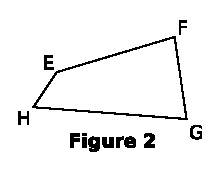
\includegraphics[width=2.8cm]{Q_EFGH}

\vspace{1cm}


\includegraphics[width=2.6cm]{Q_MNOP}
 \end{minipage} \\

\end{activite}


%%%%%%%%%%%%%%%%%%%%%%%%%%%%%%%%%%%%%%%%%%%%%%%%%%%%%%%%%%%%%%%%%%

\begin{activite}[Une figure à main levée \ldots à l'œil ouvert]
Un professeur demande à ses élèves de tracer les croquis d'un parallélogramme $ABCD$ tel que $AD = 4$ cm, $DC = 7$ cm, $\widehat{ADC} = 72^\circ$. Voici les croquis de cinq élèves : \\[0.5cm]
\begin{tabularx}{0.8\textwidth}{ccccc}
 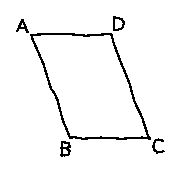
\includegraphics[width=2.3cm]{croquis_1} & 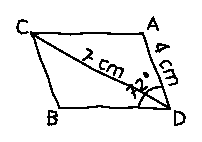
\includegraphics[width=2.7cm]{croquis_2} & 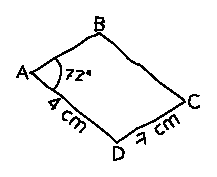
\includegraphics[width=2.8cm]{croquis_3} & 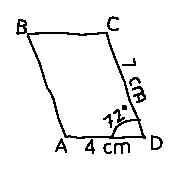
\includegraphics[width=2.3cm]{croquis_4} & 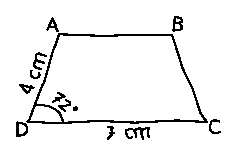
\includegraphics[width=3.1cm]{croquis_5} \\
 Rachid & Élodie & Anissa & Véronique & Patrick \\
\end{tabularx} \\


\begin{enumerate}

\item Qui a fait un croquis correct ? Pour les croquis non corrects, explique l'erreur commise.

\item Construis le parallélogramme $ABCD$.
\end{enumerate}

\end{activite}

%%%%%%%%%%%%%%%%%%%%%%%%%%%%%%%%%%%%%%%%%%%%%%%%%%%%%%%%%%%%%%%%%%

\newpage

\begin{activite}[Puzzle de Sam Lloyd]

\begin{partie}[Construction du puzzle]

\begin{minipage}[c]{0.3\linewidth}
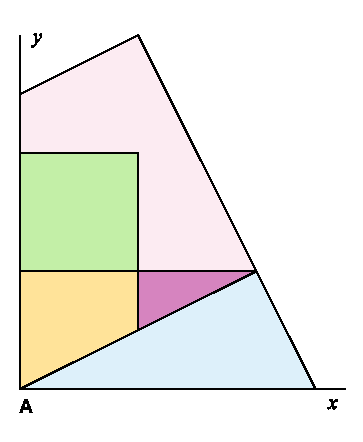
\includegraphics[width=5.2cm]{puzzle}
\end{minipage} \hfill%
\begin{minipage}[c]{0.56\linewidth}
 
  \begin{itemize}
   \item Construis deux demi‑droites perpendiculaires $[Ax)$ et $[Ay)$, puis trace le cercle de centre $A$ et de rayon 7,5 cm. Il coupe $[Ax)$ en $B$ et $[Ay)$ en $C$ ;
   \item Sur $[AC]$, place les points $E$ et $F$ tels que $AE = EF = 3$ cm ;
   \item Trace la perpendiculaire à $(AE)$ passant par $E$ et place les points $G$ et $H$ sur cette droite tels que : $EG = GH = 3$ cm ;
   \item Trace $(BH)$, puis la perpendiculaire à $(BH)$ passant par $C$. Elle coupe $(BH)$ en $J$ ;
   \item Trace $[AH]$ ;
   \item Trace la droite $d_1$ perpendiculaire à $(AE)$ passant par $F$, puis la perpendiculaire à $(EH)$ passant par $G$ qui coupe $[AH]$ en $I$ et $d_1$ en $K$.
   \end{itemize}

\end{minipage} \\

 \end{partie}

Gomme les traits de construction afin de ne conserver que ceux du modèle ci‑dessus.
   
Découpe les cinq pièces du puzzle. 

\begin{partie}[Utilisation du puzzle]
Utilise toutes les pièces du puzzle pour former un carré, un rectangle et un parallélogramme. Construis une solution sur ton cahier pour chacune des formes demandées.
 \end{partie}
 
\end{activite}
